\documentclass[a4paper, 10pt, danish, final]{article}
\usepackage{bonde}

\def\mytitle{Dataanalyse 2010}
\def\mysubtitle{Aflevering af ugeopgave 2}
\def\myauthor{Ulrik Bonde}
\def\mymail{\mailto{bonde@diku.dk}}
\def\mydate{\today}
\def\repository{\url{http://github.com/bonde/dataanalyse}}

\title{\mytitle}
\subtitle{\mysubtitle}

\author{\myauthor{} - \mymail}
\date{\mydate}

\hypersetup{
colorlinks,%
citecolor=black,%
filecolor=black,%
linkcolor=black,%
urlcolor=black,%
bookmarksopen=false,
pdftitle={\mytitle{} - \mysubtitle},
pdfauthor={\myauthor}
}

\begin{document}
\maketitle

\subsection*{Spørgsmål 1}
Jeg vil i denne opgave bruge et meget simpelt billede til at illustrere
den to-dimensionelle Fouriertransformation og effekten af ideel
filtrering af billeder. Billedet er vist i figur \ref{square} og er en
hvid firkant på en sort baggrund.

\begin{figure}[!h]
    \centering
    
\includegraphics[angle=0,width=0.45\textwidth]{images/square}
    \caption[]{Billedet som vi vil arbejde med. Motivet et simpelt og
    der er skarpe kontraster.}
    \label{square}
\end{figure}

Vi vil nu gerne finde billedets Fouriertransformation og vise det med og
uden translation af Origo til billedets midte. Fremgangsmåden er vist i
kodeboks \ref{fft_matlab} og de resulterende billeder er vist i figur
\ref{ffts}. I begge fremstillinger ses et tydeligt mønster, men først
når Origo translateres til midten bliver selve $sinc$-funktionen
åbenlys.

\begin{lstlisting}[caption={Fouriertransformation i MATLAB},
    captionpos=b, label={fft_matlab}, float=t, numbers=none]
% Read and show the original image
[I, cmap] = imread('../images/square.tiff', 'tiff');
figure; imshow(I, cmap);

% Show Fourier transform without shift
figure; imshow(log(abs(fft2(I))), cmap);

% Show Fourier transform with shift
figure; imshow(log(abs(fftshift(fft2(I)))), cmap);
\end{lstlisting}

\begin{figure}[!h]
    \centering
    \subfloat[Styrkespektret uden translation af Origo]{\label{fft_noshift}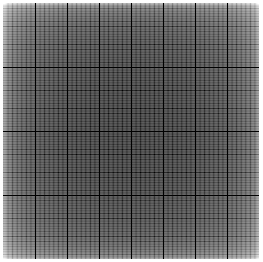
\includegraphics[angle=0,width=0.45\textwidth]{images/fft_noshift}\hspace{1em}}
    \subfloat[Styrkespektret med translation af Origo til
    billedecenteret]{\label{fft_shift}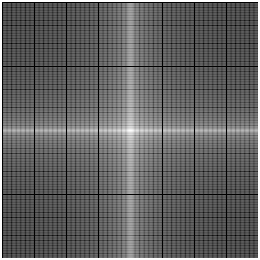
\includegraphics[angle=0,width=0.45\textwidth]{images/fft_shift}}
    \caption[]{To forskellige visninger af den samme
    Fouriertransformation. Billedet til venstre viser det egentlige
    output fra metoden \texttt{fft2} i MATLAB. Billedet til højre er
    blevet justeret således at vi har Origo i billedets midte.
    Billederne er lavet som vist i kodeboks \ref{fft_matlab}.}
    \label{ffts}
\end{figure}

Vi ønsker nu at filtrere billedet med et ideelt lav-pas-filter. Dette er
ligetil at gøre i frekvensdomænet, da vi blot kan skære de uønskede
frekvenser væk. Til filtrering er der vedlagt to MATLAB programmer.
\texttt{DAIdealFilter} opretter og returner det ideelle filter. Filteret
er defineret i frekvensdomænet og er blot en hvid cirkel som angiver
hvilke frekvenser vi lader passere.

Vi kan folde billedet og filteret i steddomænet ved at lave punktvis
multiplikation i frekvensdomænet. \texttt{DAFilterF} gør dette lettere,
da denne funktion tager et billede og et frekvensfilter. Herefter
Fouriertransformeres billedet og Origo translateres til midten. Nu
udføres den punktvise multiplikation og resultatets Origo translateres
tilbage. Endeligt laves den inverse Fouriertransformation på resultatet.
Billedet er nu blevet filteret med det givne filter.

I figur \ref{ideal_filter} er det vist og forklaret hvodan filtrering
med idealfilteret påvirker billedet.

\begin{figure}[!h]
    \centering
    \subfloat[Filter med $D_0 = 64$.]{\label{ideal_filter_64}
\includegraphics[angle=0,width=0.30\textwidth]{images/ideal_filter_64}}\hspace{1em}
    \subfloat[Filtreret frekvensdomæne]{\label{ideal_fft_64}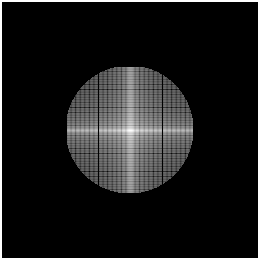
\includegraphics[angle=0,width=0.30\textwidth]{images/ideal_fft_64}}\hspace{1em}
    \subfloat[Filtreret billede]{\label{ideal_64}
\includegraphics[angle=0,width=0.30\textwidth]{images/ideal_64}}\\
    \subfloat[Filter med $D_0 = 32$.]{\label{ideal_filter_32}
\includegraphics[angle=0,width=0.30\textwidth]{images/ideal_filter_32}}\hspace{1em}
    \subfloat[Filtreret frekvensdomæne]{\label{ideal_fft_32}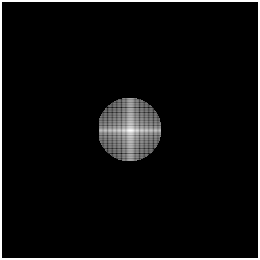
\includegraphics[angle=0,width=0.30\textwidth]{images/ideal_fft_32}}\hspace{1em}
    \subfloat[Filtreret billede]{\label{ideal_32}
\includegraphics[angle=0,width=0.30\textwidth]{images/ideal_32}}\\
    \subfloat[Filter med $D_0 = 64$.]{\label{ideal_filter_16}
\includegraphics[angle=0,width=0.30\textwidth]{images/ideal_filter_16}}\hspace{1em}
    \subfloat[Filtreret frekvensdomæne]{\label{ideal_fft_16}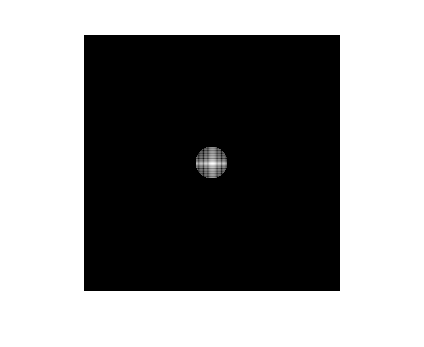
\includegraphics[angle=0,width=0.30\textwidth]{images/ideal_fft_16}}\hspace{1em}
    \subfloat[Filtreret billede]{\label{ideal_16}
\includegraphics[angle=0,width=0.30\textwidth]{images/ideal_16}}
    \caption[]{Tre forskellige filtreringer med idealfilteret med
    $D_0$ sat til hhv. 64, 32 og 16. Ved første filter ses det allerede
    at de skarpe kontraster udlignes ved brug af idealfilteret. Kanterne
    på firkanten bliver slørede og der ses ring-effekt. Dette
    intensiveres når $D_0$ bliver mindre, dvs. vi skærer flere høje
    frekvenser væk. Det ses at meget at billedeinformationen ligger i de
    lave frekvenser, da vi ved en lille værdi af $D_0$ stadig har en god
    fornemmelse af hvad billedet forestiller. Til at illustrere dette
    kunne man godt have brugt et andet billede.}
    \label{ideal_filter}
\end{figure}
\clearpage

\subsection*{Spørgsmål 2}


%%%%%%%%%%%%%%%%%%%%%%%%%%%%%%%%%%%%%%%%%%%%%%%%%%%%%%%%%%%%%%%%%%%%
% Formal stuff

%\bibliographystyle{abbrvnat}
%\bibliography{bibliography}
%\addcontentsline{toc}{chapter}{Litteratur}

\appendix
\lstset{language=Matlab, basicstyle=\scriptsize,
    showstringspaces=false, numbers=left, stepnumber=1,
    numberstyle=\tiny, frame=none}
\section{Kildekode}
Kildekoden er tilgængelig i mit git-repository på \repository{}. Bemærk
at prefikset \texttt{DA} står for ``DataAnalyse'' og blot er til for at
undgå eventuelle sammenstød med indbyggede funktioner i MATLAB.

\subsection{DAIdealFilter.m}
\lstinputlisting{../src/DAIdealFilter.m}

\subsection{DAFilterF.m}
\lstinputlisting{../src/DAFilterF.m}

\end{document}

% vim: set tw=72 spell spelllang=da:
